\subsection{Frozen-component interventions on reached BE states}\label{sec:components}
We select all three BE seeds with any functional failure in the 40-model
study, retain both arms and all 1,000 original cases per model, and compare
five fixed modes: unchanged policy; exact KW confirmation on actual learned
messages; exact KW participation with learned proposal/COMMIT recomputed;
first-free KW candidates with learned participation/COMMIT recomputed; and
all three exact KW components. Learned Linial decisions remain unchanged.
This is a retrospective diagnostic on consumed cases, selected by known
failures, not a new training-method test. Its protocol and source/weight
hashes are frozen before replay outcomes. All baseline terminal vectors,
statuses, steps and invariant flags must reproduce before interpreting
interventions. The other learned modules retain their weights; their later
outputs are recomputed after trajectories diverge.
The exact KW predicate uses each reached state's valid auxiliary coloring,
clock and bounds; it is the diagnostic state-domain extension specified
with the contracts, not an assumption that every rollout state is an exact
teacher prefix.

All six unchanged baselines reproduce the original 6,000 terminal vectors,
statuses, step counts and invariant flags exactly. Across the 30,000
executions there are no technical errors and no newly failed cases under
an intervention. In CF seeds 105001 and 105008, exact COMMIT alone raises
successes from 100 and 101 to 1,000 each, rescuing all 900 and 899 failures.
Changing only participation or candidates rescues none. All 1,312 and 1,322
missed valid writes reached by their unchanged policies occur at
$\kappa=0$; unlike the 181 teacher-prefix false negatives, some have
participating neighbors (358 and 406). These are visit counts, not
independent errors or new training replicas.

In seed 105010, both arms complete 204/1,000. Exact COMMIT or candidates
alone leave all 796 failures unchanged. Exact participation alone rescues
all 796 in each arm; the unchanged policy is silent on 983 eligible reached
queries. All-exact KW modules yield 1,000/1,000 for each of the six models,
while learned Linial modules remain fixed. Thus COMMIT-only rescues 1,799
of the 2,595 CF failures on this original battery, and participation-only
rescues the remaining 796. Counts across arms share cases and first-stage
tensors; they are not independent intervention replications.

\begin{figure}[htbp]\centering
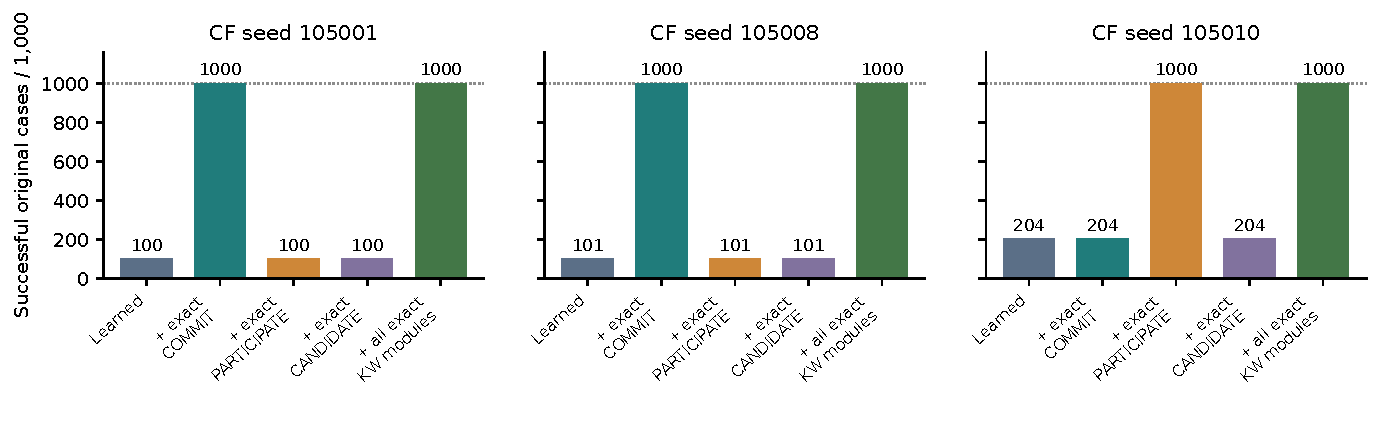
\includegraphics[width=\linewidth]{figures/integration-functional-components.pdf}
\caption{Component interventions on the three selected CF seeds, using all
original cases. Each replacement changes one KW component and recomputes
dependent learned outputs on the ensuing trajectory. All-exact replaces
three KW components. These retrospective diagnostic successes do not
establish a learned repair or general intervention success rate. Native
arms and case-level outputs are retained in Appendix~\ref{app:integration}.}
\label{fig:components}
\end{figure}


The interventions use oracle decisions and are diagnostic tools, not deployable
learned policies. Their fixed-battery rescue counts localize mechanisms in
the selected models; they do not estimate a population remedy. Errors on
teacher-prefix continuation queries and errors reached during autonomous
rollouts have different denominators and are reported separately.
